% Capa
\begin{titlepage}
% Se quiser uma figura de fundo na capa ative o pacote wallpaper
% e descomente a linha abaixo.
% \ThisCenterWallPaper{0.8}{nomedafigura}

\begin{center}
{\large \textbf{UNIVERSIDADE FEDERAL DO ESPÍRITO SANTO \\ CENTRO TECNOLÓGICO \\ PROGRAMA DE PÓS-GRADUAÇÃO EM INFORMÁTICA}}
\par
\vspace{120pt}
{\LARGE \textbf{MARCOS ALÉCIO SPALENZA}}

\par
\vspace{160pt}
{\LARGE \textbf{APLICAÇÃO DE SELEÇÃO DE CARACTERÍSTICAS PARA MELHORIA DE UM SISTEMA SEMIAUTOMÁTICO DE AVALIAÇÃO DE QUESTÕES DISCURSIVAS}}
\par
\vfill
\textbf{{\large VITÓRIA-ES}\\
{\large 2017}}
\end{center}
\end{titlepage}

% A partir daqui páginas sem cabeçalho
\pagestyle{empty}
% Faz com que a página seguinte sempre seja ímpar (insere pg em branco)
\cleardoublepage

% Números das páginas em algarismos romanos
\pagenumbering{roman}









%Capa2
\newpage
\begin{center}
% Acerte as distâncias de acordo com o seu nome e o título da sua tese ou
% dissertação
{ \bfseries\fontsize{13}{15}\selectfont
\rotatebox{90}{\hspace{3cm}MARCOS ALÉCIO SPALENZA \hspace{3cm} Dissertação de MESTRADO
 \hspace{0.8cm} - 2017
\hspace{0.5cm} } }
\end{center}










% Página de Rosto
\newpage
\begin{center}
{\LARGE \textbf{MARCOS ALÉCIO SPALENZA}}
\par
\vspace{200pt}
{\LARGE \textbf{APLICAÇÃO DE SELEÇÃO DE CARACTERÍSTICAS PARA MELHORIA DE UM SISTEMA SEMIAUTOMÁTICO DE AVALIAÇÃO DE QUESTÕES DISCURSIVAS}}
\end{center}
\par
\vspace{90pt}
\hspace*{175pt}\parbox{10cm}{{Dissertação apresentada ao Programa de Pós-Graduação em Informática do Centro Tecnológico da Universidade Federal do Espírito Santo, como requisito parcial para a obtenção de Título de Mestre em Informática.}}

\par
\vspace{1em}
\hspace*{175pt}\parbox{10cm}{{Orientador: Prof. Dr. Elias de Oliveira}\\{Co-orientador: Profª. Dr. Márcia Gonçalves de Oliveira}}
 %Co-orientador: Prof. Dr. Patrick M. Ciarelli 

\par
\vfill
\begin{center}
\textbf{{\large VITÓRIA-ES}\\
{\large 2017}}
\end{center}









%Ficha Catalográfica
\newpage
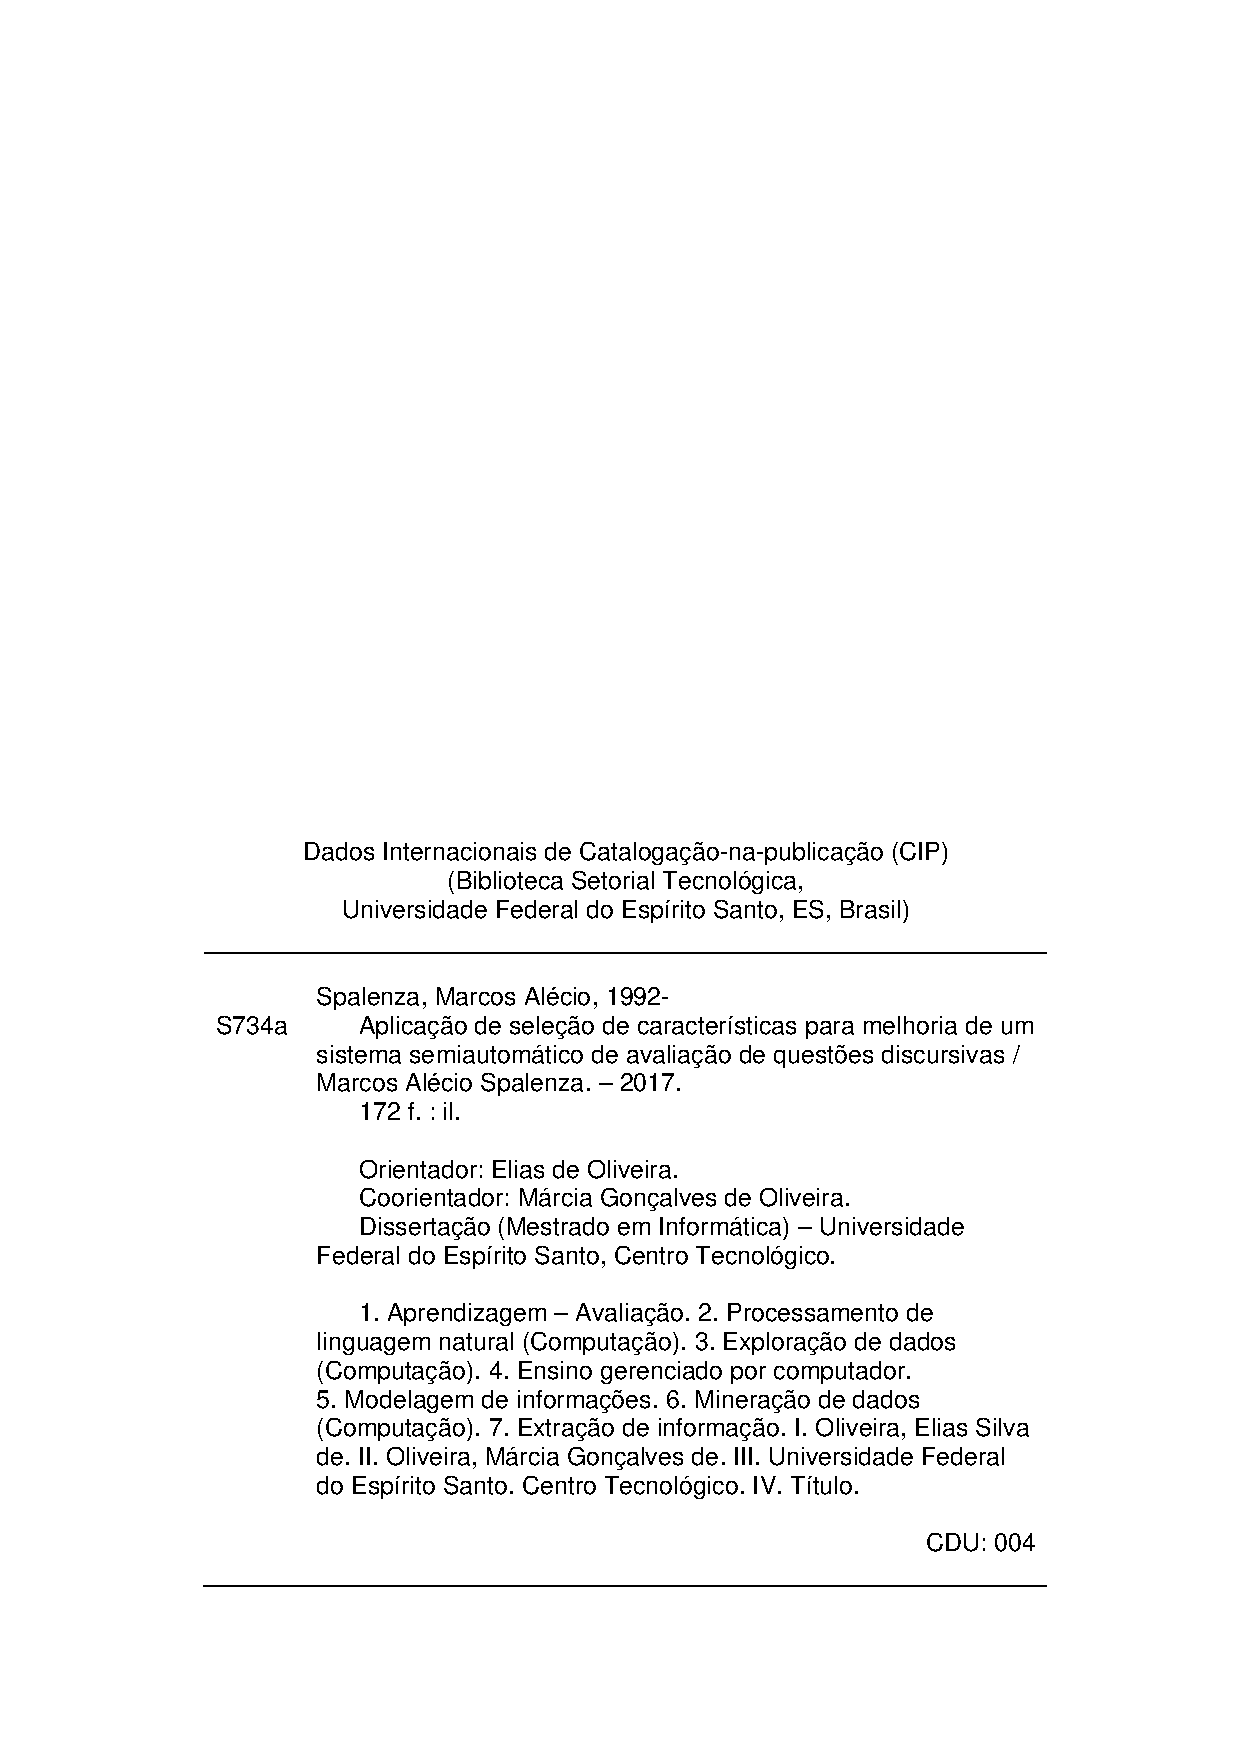
\includepdf{tables/ficha-catalografica.pdf}










%Folha de Aprovação
\newpage
\begin{center}

{%
\bfseries
\fontsize{14}{16}\selectfont
MARCOS ALÉCIO SPALENZA
}
\vspace{0.5cm}

{
\bfseries
\fontsize{15}{17}\selectfont
\MakeUppercase{{APLICAÇÃO DE SELEÇÃO DE CARACTERÍSTICAS EM UM SISTEMA SEMIAUTOMÁTICO DE AVALIAÇÃO DE QUESTÕES DISCURSIVAS}}\\
}

\vspace{0.5cm}
\end{center}
{
\fontsize{12}{14}\selectfont
Dissertação submetida ao programa de Pós-Graduação em Informática do Centro Tecnológico da Universidade Federal do Espírito Santo, como
requisito parcial para a obtenção do Grau de Mestre em Informática.}

%\vspace{0.1cm}

\begin{flushright}
{
\fontsize{12}{14}\selectfont
Aprovada em 20 de abril de 2017.}
\end{flushright}

\vspace{0.5cm}

%\begin{flushright}
\begin{quote}
{
\bfseries
\fontsize{16}{18}\selectfont
\hspace{3cm}COMISSÃO EXAMINADORA
}
\vspace{0.8cm}
{
\fontsize{11}{13}\selectfont

%\begin{singlespace}
\hspace*{3cm}\rule{105mm}{0.2mm}\\
\hspace*{3cm}Prof. Dr. Elias de Oliveira\\
\hspace*{3cm}Universidade Federal do Espírito Santo \\
\hspace*{3cm}Orientador\\
\hspace*{3cm}\rule{105mm}{0.2mm}\\
\hspace*{3cm}Profª. Dr. Márcia Gonçalves de Oliveira\\
\hspace*{3cm}Centro de Referência em Formação e em Educação a Distância\\
\hspace*{3cm}Co-orientadora\\ 
\hspace*{3cm}\rule{105mm}{0.2mm}\\
\hspace*{3cm}Prof. Dr. Davidson Cury\\
\hspace*{3cm}Universidade Federal do Espírito Santo\\[0.5cm]
\hspace*{3cm}\rule{105mm}{0.2mm}\\
\hspace*{3cm}Prof. Dr. Pável Calado\\
\hspace*{3cm}Instituto de Engenharia de Sistemas e Computadores - Investigação \hspace*{3cm}e Desenvolvimento em Lisboa\\[1ex]

%\end{singlespace}
}
\end{quote}













\newpage
% Dedicatória
% Posição do texto na página
\vspace*{\fill}
\begin{flushright}
  \emph{Dedico esse trabalho aos meus pais, Marcos e Sirlene, e ao meu irmão, Murilo, pelo apoio em todos os momentos, inclusive durante esse tempo de imersão nos estudos.\\ Sem a ajuda deles, nada seria possível.}
\end{flushright}



















\newpage
% Agradecimentos

% Espaçamento duplo
\vspace*{4cm}

%\begin{center}
{
\bfseries
\fontsize{18}{22}\selectfont
Agradecimentos
}

\vspace*{0.5cm}
%\end{center}

Agradeço a Deus.

Agradeço aos meus pais, Marcos e Sirlene, pela oportunidade e suporte incondicional.

Agradeço ao meu irmão, Murilo, pela grande amizade e por me apoiar sendo sempre presente.

Agradeço meus tios, Vanderlei e Solange, que muito me ajudaram, possibilitando meus estudos em Vitória.

Minha gratidão ao Professor Elias de Oliveira, pela disponibilidade e por cada orientação acreditando no andamento desse trabalho. 

Agradeço a Professora Márcia Gonçalves de Oliveira, por todas orientações, contribuições e dicas.

Agradeço a todos os amigos, principalmente os que fiz durante o mestrado, por cada conversa, incentivo e desafio passados.

Agradeço a todos os membros do PPGI e do LCAD, pelo suporte, pelos conhecimentos adquiridos e pelo profissionalismo ímpar.

Também sou grato à todos que fizeram parte, direta ou indiretamente, da minha formação.

\newpage
%Epígrafe
\begin{flushright}
\vspace{17cm}
\vspace*{0.75\textheight}
\textit{``I don't believe in pessimism. If something doesn't come up the way you want, forge ahead. If you think it's going to rain, it will.''\\
(Clint Eastwood)}
\end{flushright}
















\newpage
%Publicações
% Espaçamento duplo
\doublespacing

\noindent{\LARGE\textbf{Publicações}}

\par Como parte desse trabalho, foram desenvolvidos e publicados os seguintes trabalhos, no período do mestrado, que apresentam, em maior ou menor grau, relação com o tema proposto.

%\par Publicação em revista:
%\begin{itemize}
%\item Saúde, M. R.; Soares, M. M.; Ciarelli, P. M.; Oliveira, E. %\textbf{Seleção de características aplicada à moderação automática de %comentários de usuários}. Revista Eletrônica Científica Inovação e %Tecnologia. Universidade Federal Tecnológica do Paraná. Campus %Medianeira. No prelo (2014). ISSN 2175-1846.
%\end{itemize}

\par Publicação de trabalhos em anais de congressos:
\begin{itemize}
\itemsep=-.3mm

\item Spalenza, M. A.; Nogueira, M. A.; Oliveira, M. G.; Oliveira, E. \textbf{Uso de Mapa de Características na Avaliação de Textos Curtos nos Ambientes Virtuais de Aprendizagem}. XXVII Simpósio Brasileiro de Informática na Educação (SBIE). Uberlândia, MG, Brazil. 2016.

\item Spalenza, M. A.; Nogueira, M. A.; Oliveira, M. G.; Oliveira, E. \textbf{Construção de Mapas de Características em Classes de Respostas Discursivas}.  XXI Congreso Internacional de Informática Educativa (TISE). Santiago, Chile. 2016.

\end{itemize}








\newpage
\vspace*{10pt}
% Abstract
\begin{center}
  \emph{\begin{large}Resumo\end{large}}\label{resumo}
\vspace{2pt}
\end{center}
% Pode parecer estranho, mas colocar uma frase por linha ajuda a organizar e reescrever o texto quando necessário.
% Além disso, ajuda se você estiver comparando versões diferentes do mesmo texto.
% Para separar parágrafos utilize uma linha em branco.

O processo de avaliação é muito importante para a verificação de aprendizagem dos estudantes e manutenção do andamento do ensino conforme o currículo previsto. A avaliação formativa, garante ao professor a visão geral do ensino de forma a medir a efetividade do aprendizado. Porém, conforme é ampliado o acesso à educação, a aplicação de métodos avaliativos se torna ainda mais necessária e a carência de apoio em sua aplicação é vista como um fator limitante.

O suporte computacional dos métodos pedagógicos visa melhorar a qualidade dos materiais para impactar diretamente na aprendizagem. Neste trabalho, apresentamos uma ferramenta de apoio à correção de respostas discursivas curtas segundo os termos e sua respectiva representatividade por classe de nota. A adoção da seleção de características proporciona a criação de modelos de avaliação mais próximos ao critério do professor. Com os trechos de respostas identificados esperamos padrões que tornem o sistema um avaliador em potencial. Assim, o conjunto da modelagem do método avaliativo e seu \textit{feedback} para suporte ao ensino é aqui chamada de mapas de características.

\noindent

\par
\vspace{1em}
\noindent\textbf{Palavras-chave:} Mapa de Características, Avaliação Assistida por Computador, Mineração de Dados Educacionais, Aprendizado Semiautomático, Extração de Informação.




\newpage
% Criei a página do abstract na mão, por isso tem bem mais comandos do que o resumo acima, apesar de serem idênticas.
\vspace*{10pt}
% Abstract
\begin{center}
  \emph{\begin{large}Abstract\end{large}}\label{abstract}
\vspace{2pt}
\end{center}

% Selecionar a linguagem acerta os padrões de hifenação diferentes entre inglês e português.
%\selectlanguage{english}

\begin{comment}
Automatic evaluation of free-text answers was introduced to relieve teacher overload problems supporting your evaluation methods. In the end of nineties, with student's discourse verification, arise some works based on context analysis for short text. Meanwhile, essay evaluation has focused in writting style and theme definition. Accordingly, while both are textual activities, evaluation criteria of short text answers need to be closer of teacher correction models.

In this work, we present a tool for feature selection based on term frequency and its class representativity. The dimensionality reduction provide evaluation models more similar to teacher correction criteria. With identification of answers elements, this system builds a visualization structure called features map.

Therefore, features map aims to present all key contents selected for tutor, detailling his answers database. As a consequence of summarization for answer sets, we improve the classification performance. This summaries will be send to students as question's feedback, helping with mutual comprehension about the content. Hopefully, this tool enable teachers and students to organize talks on marked answers for discussion of results and provide collaborative analysis.

\end{comment}
The evaluation process is an important step for student's learning verification to keep the teaching program as expected. The formative evaluation ensures the teacher a general view of the lesson to determine their effectiveness. Therefore, according to the improvements in education access, the evaluation methods have become increasingly needed and its support deficiency should be seen as a limiting factor.

The computational support for pedagogical methods want to improve the quality of materials causing a direct and positive impact on learning. In this work, we present a tool to supports short answer evaluation based on terms and its representativeness inside grade classes. Feature selection adoption provides models closer than teacher's criteria. With identifyed terms as patterns, turns system into a potential answer evaluator. Thus, the criteria modelling and its feedback to teaching support is called features map.

\noindent

\par
\vspace{1em}
\noindent\textbf{Keywords:} Features Map, Computer Assisted Assessment,  Educational Data Mining, Semiautomatic Learning, Information Extraction.




\clearpage
\pagestyle{headings}

%%%%%%%%%%%%%%%%%%%%%%%%%%%%%%%%%%%%%%%%%%%%%%%%%%%%%%%%%%%%%%%%%%%%%%%
% Definição do formato de cabeçalho (package fancyhdr.sty)
% Este material deveria estar em um local mais apropriado

% Definir um estilo para páginas completas (cabeçalho + rodapé)
\pagestyle{fancyplain}

% Marca de capítulo do tipo "2. Blábláblá..." no cabeçalho
\renewcommand{\chaptermark}[1]{\markboth{\thechapter.\ {#1}}{}}

% Para aumentar o tamanho da caixa para o cabeçalho
\addtolength{\headheight}{\baselineskip}

% Definindo o conteúdo do cabeçalho...
\fancyhf{}
%\fancyhead[LO,LE]{\nouppercase{\textsf{\leftmark}}}
\fancyhead[L]{\nouppercase{\textsf{\leftmark}}}
%\fancyhead[RO,RE]{\thepage}
\fancyhead[R]{\thepage}

% Para garantir que a primeira página de cada capítulo...
\fancypagestyle{plain}{%
\fancyhf{}%                         % não terá head ou foot
\renewcommand{\headrulewidth}{0pt}} % nem linhas de cabeçalho
%%%%%%%%%%%%%%%%%%%%%%%%%%%%%%%%%%%%%%%%%%%%%%%%%%%%%%%%%%%%%%%%%%%%%%%

% Capítulos são numerados normalmente
\pagenumbering{arabic}
\setcounter{page}{10}






\newpage

% Lista de figuras
\listoffigures



% Lista de tabelas
\listoftables



% Abreviações
% Para imprimir as abreviações siga as instruções em 
% http://code.google.com/p/mestre-em-latex/wiki/ListaDeAbreviaturas
%\printnomenclature

% Índice
\tableofcontents
